%% LyX 2.3.2 created this file.  For more info, see http://www.lyx.org/.
%% Do not edit unless you really know what you are doing.
\documentclass{ctexart}
\usepackage{amsmath}
\usepackage{fontspec}
\usepackage{geometry}
\geometry{verbose,tmargin=2cm,bmargin=2cm,lmargin=2cm,rmargin=2cm}
\usepackage{bm}
\usepackage[unicode=true,pdfusetitle,
 bookmarks=true,bookmarksnumbered=false,bookmarksopen=false,
 breaklinks=false,pdfborder={0 0 1},backref=false,colorlinks=false]
 {hyperref}

\makeatletter
%%%%%%%%%%%%%%%%%%%%%%%%%%%%%% User specified LaTeX commands.
%!TEX TS-program = xelatex

\usepackage[super,square,comma,sort&compress]{natbib}
\usepackage{graphicx}
\usepackage{float}
\makeatletter 
\@addtoreset{equation}{section} 
\makeatother 
\renewcommand{\theequation}{\arabic{section}.\arabic{equation}} 

\makeatother

\begin{document}
\title{有限元大作业报告}
\author{(黄轩宇,力6,2016011542)}
\date{2019.6.10}

\maketitle
\tableofcontents{}

\section{板单元(Plate Element)}

\subsection{板单元的基本公式}

我们选用的板单元为4节点Kirchoff板单元,如图\ref{f1}所示:

\begin{figure}[H]
\centering  
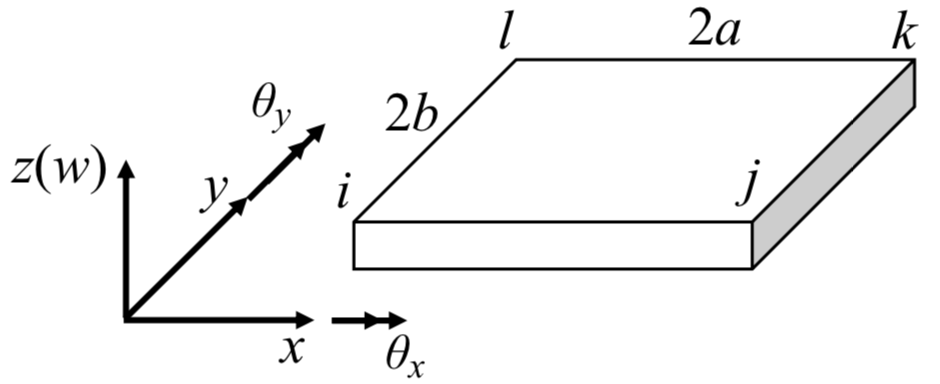
\includegraphics[width = .5\textwidth]{1.png} 
\caption{Kirchoff板单元结构示意图} 
\label{f1} 
\end{figure}

其中每一个节点具有一个垂直于板的位移自由度$w$和绕板平面内两个垂直轴,即$x$轴和$y$轴的转角$\text{\ensuremath{\theta_{x}},\ensuremath{\theta_{y}}}$,同时Kirchoff板遵循平截面和直法线假设,因此板内部的位移场为:

\begin{equation}
\begin{array}{l}
{u=u_{0}+z\theta_{y}}\\
{v=v_{0}-z\theta_{x}}\\
{w=w_{0}(x,y)}
\end{array}\label{eq1}
\end{equation}

其中转角和挠度的关系为:

\begin{equation}
\theta_{x}=\frac{\partial w}{\partial y},\quad\theta_{y}=-\frac{\partial w}{\partial x}\qquad\gamma_{xz}=\gamma_{yz}=0\label{eq2}
\end{equation}

代入到应变和转角的关系中可以得到:

\begin{equation}
\boldsymbol{\varepsilon}=\left\{ \begin{array}{c}
{\varepsilon_{x}}\\
{\varepsilon_{y}}\\
{\gamma_{xy}}
\end{array}\right\} =z\left\{ \begin{array}{c}
{-\frac{\partial^{2}w}{\partial x^{2}}}\\
{-\frac{\partial^{2}w}{\partial y^{2}}}\\
{-2\frac{\partial^{2}w}{\partial x\partial y}}
\end{array}\right\} \label{eq3}
\end{equation}

可见在此假设下板单元的应力场只有三个分量

\subsection{板单元的应力应变以及刚度阵构造}

由公式(\ref{eq3})再代入应力应变关系中可以得到:

\begin{equation}
\left[\begin{array}{c}
{\sigma_{x}}\\
{\sigma_{y}}\\
{\tau_{xy}}
\end{array}\right]=\frac{E}{1-v^{2}}\left[\begin{array}{ccc}
{1} & {v} & {0}\\
{v} & {1} & {0}\\
{0} & {0} & {\frac{1-v}{2}}
\end{array}\right]\left[\begin{array}{c}
{\varepsilon_{x}}\\
{\varepsilon_{y}}\\
{\gamma_{xy}}
\end{array}\right]\label{eq4}
\end{equation}

由于三个应力分量和坐标$z$呈现线性关系,因此进行积分得到相应的力矩:

\begin{equation}
\begin{aligned}M & =\left\{ \begin{array}{l}
{M_{x}}\\
{M_{y}}\\
{M_{xy}}
\end{array}\right\} =\boldsymbol{D}\boldsymbol{\kappa}=\boldsymbol{D}\boldsymbol{L}w\\
M_{x} & =\int_{-t/2}^{t/2}z\sigma_{x}\mathrm{d}z\\
M_{y} & =\int_{-t/2}^{t/2}z\sigma_{y}\mathrm{d}z\\
M_{xy} & =\int_{-t/2}^{t/2}z\tau_{xy}\mathrm{d}z
\end{aligned}
\label{eq5}
\end{equation}

而最终的方程:

\begin{equation}
\boldsymbol{L}^{\mathrm{T}}\boldsymbol{D}\boldsymbol{L}w-q=0\label{eq6}
\end{equation}

最后构造w的差值函数(由于每一个板单元有12个自由度,因此构造一个具有12项的三次完备多项式):

\begin{equation}
w^{e}=\bm{P}\bm{\alpha^{e}}\label{eq7}
\end{equation}
然后利用节点的位移以及转角得到:

\begin{equation}
\bm{d^{e}}=\bm{M}\bm{\alpha}^{e}\label{eq8}
\end{equation}
代入公式(\ref{eq7})可以得到:

\begin{equation}
\begin{array}{c}
w^{e}=\bm{Nd^{e}}\\
\bm{N=PM^{-1}}
\end{array}\label{eq9}
\end{equation}
进行简单的坐标变换可以得到矩形板单元的形函数表达式:

\begin{equation}
\text{\ensuremath{\bm{N^{T}}=\frac{1}{8}\begin{bmatrix}-(s-1)(t-1)(s^{2}+s+t^{2}+t-2)\\
-b(s-1)(t-1)^{2}(t+1)\\
a(s-1)^{2}(s+1)(t-1)\\
(s+1)(t-1)(s^{2}-s+t^{2}+t-2)\\
b(s+1)(t-1)^{2}(t+1)\\
a(s+1)^{2}(s-1)(t-1)\\
-(s+1)(t+1)(s^{2}-s+t^{2}-t-2)\\
b(s+1)(t+1)^{2}(t-1)\\
-a(s+1)^{2}(s-1)(t+1)\\
(s-1)(t+1)(s^{2}+s+t^{2}-t-2)\\
-b(s-1)(t+1)^{2}(t-1)\\
-a(s-1)^{2}(s+1)(t+1)
\end{bmatrix}}}\label{eq10}
\end{equation}
对形函数$\bm{N}$进行求导得到:

\begin{equation}
\bm{B}=\bm{LN}\label{eq11}
\end{equation}
相应的力矩$\text{\ensuremath{\bm{M}=\bm{DBd^{e}}}}$,从而我们得到单元刚度阵(单元的长,宽分别为$2a,2b$):

\begin{equation}
\bm{K}=ab\int_{-1}^{1}\int_{-1}^{1}\bm{B^{T}DB}{\rm d}s{\rm d}t\label{eq12}
\end{equation}
将公式(\ref{eq10})和公式(\ref{eq11})代入(\ref{eq12})中,并用matlab进行符号运算得到刚度阵的元素,然后利用skyline的存储方式输入到Stap++的Plate类的单元Stiffmatrix函数中

\subsection{应力计算以及后处理}

将单元刚度阵组装之后计算得到整体刚度阵中板单元的贡献;于此同时,对受力进行等效到节点上:

\begin{equation}
f_{i}=\left\{ \begin{array}{l}
{f_{w_{i}}}\\
{f_{\theta_{i_{i}}}}\\
{f_{\theta_{i_{i}}}}
\end{array}\right\} =\int_{-b}^{b}\int_{-a}^{a}N^{\mathrm{T}}q\mathrm{d}x\mathrm{d}y\label{eq13}
\end{equation}
对于重力的作用:$q=\rho gt$($t$为板单元的厚度,$\rho$为材料密度,$g$为重力加速度),代入公式(\ref{eq13})可以得到:

\begin{equation}
\begin{array}{l}
{f_{1z}=-\frac{1}{12}\rho gtab\left\{ \begin{array}{c}
{3}\\
{b}\\
{-a}
\end{array}\right\} \quad f_{2}=-\frac{1}{12}\rho gtab\left\{ \begin{array}{c}
{3}\\
{-b}\\
{-a}
\end{array}\right\} }\\
{f_{3}=-\frac{1}{12}\rho gtab\left\{ \begin{array}{l}
{3}\\
{b}\\
{a}
\end{array}\right\} \quad f_{4}=-\frac{1}{12}\rho gtab\left\{ \begin{array}{c}
{3}\\
{-b}\\
{a}
\end{array}\right\} }
\end{array}\label{eq14}
\end{equation}
同样将其组装到整体的方程中,可以求解相应的节点位移和转角。

利用求解得到的位移和转角代入公式(\ref{eq9})中可以得到相应的挠度分布,仅以不由转角-挠度关系(\ref{eq2})可以得到单元内部的转角分布

关于应力,由(\ref{eq3})可知:应力和应变在中性面的值为0,在表面最大,因此我们可以选择输出表面的应力$(z=\pm\frac{t}{2})$或者$z$方向高斯点$(z=\pm\frac{t}{2\sqrt{3}})$的应力:

\begin{equation}
\begin{array}{cc}
\text{表\text{面}} & \bm{\sigma_{(\pm)}^{e}=}\pm\frac{6}{t^{2}}\bm{M^{e}}\\
Gauss\text{点} & \bm{\sigma_{(\pm)}^{e}=}\pm\frac{6}{\sqrt{3}t^{2}}\bm{M^{e}}
\end{array}\label{eq15}
\end{equation}
最后针对后处理的输出,可以输出相应上下表面对应xy平面的Gauss点的Mises应力,然后取其平均值作为该单元的Mises应力。

\subsection{输入文件格式和自由度约束}

主体的输入文件格式基本不变,但是对于板单元而言,其节点只有三个自由度,也就是说其另外三个自由度是锁死的,那么对于倾斜的板单元,其对应的约束就较为复杂,需要利用旋转刚度阵将其进行坐标变换,由于最终的桥梁算例中,板单元都是位于xy平面内的,因此在Stap++中并没有实现倾斜板的功能;在此情况下输入文件中6个bcode数中,前两个(bcode{[}0{]},bcode{[}1{]})和最后一个(bcode{[}5{]})都应该设为1,而其余几个bcode数则根据具体的模型约束情况而定,我们以一个板单元的输入文件为例子,如图\ref{f2}所示:

\begin{figure}[H]
\centering  
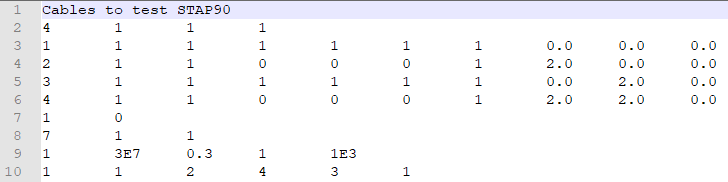
\includegraphics[width = .8\textwidth]{2.png} 
\caption{1个单元的板单元输入文件示意图} 
\label{f2} 
\end{figure}

而后续的节点力则按照公式(\ref{eq14})添加,格式和其他单元一致。

\subsection{分片测试}

我们在$[-1,1]^{2}$的正方形板构造这样的位移场 $w=x^{2}-\nu y^{2}$, 由公式(\ref{eq2})可以得到:

\begin{equation}
\begin{array}{c}
\theta_{x}=-2\nu y\\
\theta_{y}=-2x
\end{array}\label{eq16}
\end{equation}
由公式(\ref{eq5})可以得到均匀弯矩场:

\begin{equation}
\bm{M^{e}=}\begin{bmatrix}-\frac{1}{6}Et^{3}\\
0\\
0
\end{bmatrix}\label{eq17}
\end{equation}
其中$E=30,\nu=0.2,t=1$;利用$x=0$;$y=0$;$y=0.5$三条直线 将正方形板分割成六个分片,如图\ref{f3}所示:

\begin{figure}[H]
\centering  
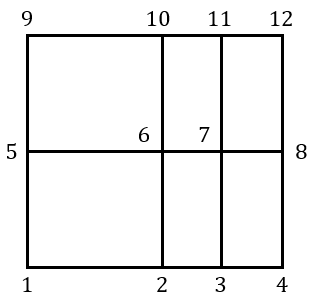
\includegraphics[width = .3\textwidth]{3.png} 
\caption{Plate单元分片实验划分示意图} 
\label{f3} 
\end{figure}

对应的将法线沿 x 轴方向边界($x=\pm1$)上的 y 向弯矩分配到边界上的每个点上:

\begin{equation}
\begin{array}{c}
M_{4y}=-M_{1y}=-2.5\\
M_{8y}=-M_{5y}=-5\\
M_{12y}=-M_{9y}=-2.5
\end{array}\label{eq18}
\end{equation}

具体输入文件见 Platepatchtest,dat,在程序中的位移输出结果如图\ref{f4}所示:

\begin{figure}[H]
\centering  
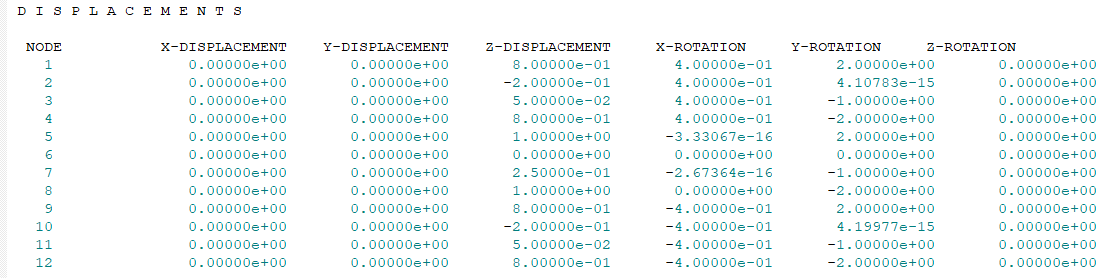
\includegraphics[width = .9\textwidth]{4.png} 
\caption{Plate单元分片实验位移结果} 
\label{f4} 
\end{figure},可见位移$w$准确,误差在浮点数范围内,以7号节点为例:

\begin{equation}
\begin{array}{c}
w_{7}=x_{7}^{2}-\nu y_{7}^{2}=0.25\\
\theta_{x7}=-2\nu y_{7}=0\\
\theta_{y7}=-2x_{7}=-1
\end{array}\label{eq19}
\end{equation}
从$\theta_{x}$上的误差上来看,误差基本上在$10^{-16}$量级上,为计算机浮点数的误差

\subsection{收敛率计算}

考虑一个正方形板,$W=L=2,t=1$,其中$E=3\times10^{7},\nu=0.3,t=1$如图\ref{f5}所示:

\begin{figure}[H]
\centering  
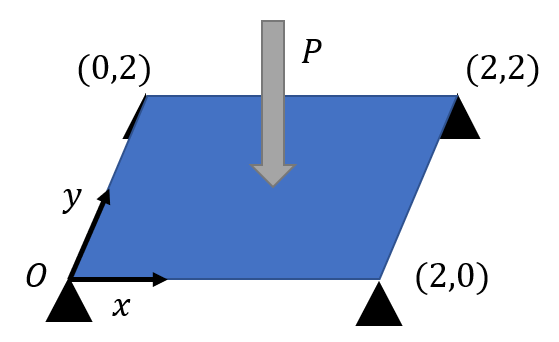
\includegraphics[width = .5\textwidth]{5.png} 
\caption{Plate收敛率计算示意图} 
\label{f5} 
\end{figure}在中心点施加一个集中力($-z$方向)$P=10^{5}$,因此只需要在对应的节点施加这样一个力即可,然后分别考虑划分4,16,64和256个等大小的矩形板单元进行计算(对应单元尺寸$h=1,0,5,0.25,0.0.125$),相应的输入文件用data.m生成,分别为:Plate4ele.dat,Plate16ele.dat和Plate64ele.dat,Plate256ele.dat,计算相应的节点位移$w^{e}$与理论结果进行比较:

\begin{equation}
w=\frac{16P}{D\pi^{4}}\sum_{m=0}^{\infty}\sum_{n=0}^{\infty}\frac{(-1)^{(}m+n)}{\left((2m+1)^{2}+(2n+1)^{2}\right)^{2}}\sin\frac{m\pi x}{2}\sin\frac{n\pi y}{2}\label{eq20}
\end{equation}
计算误差范数:

\begin{equation}
error=(\int_{0}^{L}\int_{0}^{W}(w^{e}-w)^{2}dxdy)^{\frac{1}{2}}\label{eq21}
\end{equation}
由于$w$至少是4次场,所以该积分至少需要采用16{*}16的Gauss积分才能准确积分,得到计算结果如图\ref{f6}所示,并作出误差范数和单元尺寸的对数图

\begin{figure}[H]
\centering  
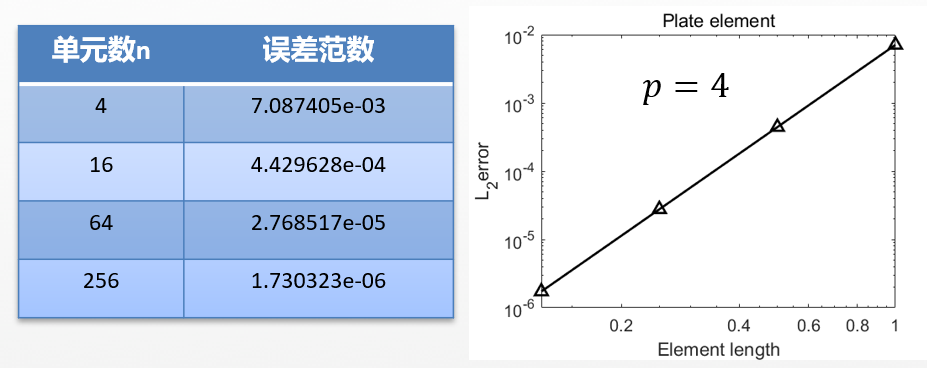
\includegraphics[width = .5\textwidth]{6.png} 
\caption{Plate收敛率计算结果} 
\label{f6} 
\end{figure}可见板单元的挠度$w$是4阶收敛的,因为其构造挠度的多项式是3次完备的。

\section{9节点平面亚参元(Subparameter Element)}

\subsection{9节点平面亚参元基本公式}

我们这里采用的9节点平面亚参元,其母单元示意图如图\ref{f7}所示:

\begin{figure}[H]
\centering  
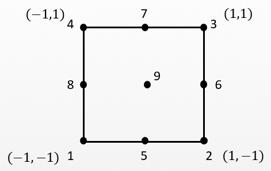
\includegraphics[width = .5\textwidth]{7.png} 
\caption{9节点平面亚参元母单元示意图} 
\label{f7} 
\end{figure}其坐标差值点为1,2,3,4四个节点,而位移差值采用1-9九个节点:

\begin{equation}
\begin{aligned}x & =\sum_{I=1}^{4}N_{I}^{\prime}x_{I}\\
y & =\sum_{I=1}^{4}N_{I}^{\prime}y_{I}\\
\theta & =\sum_{K=1}^{9}N_{K}\theta_{K}
\end{aligned}
\label{eq22}
\end{equation}
其中$N_{I}^{\prime}=\frac{1}{4}\left(1+\xi_{I}\xi\right)\left(1+\eta_{I}\eta\right)$,而:

\begin{equation}
\begin{array}{c}
N_{1}=\frac{1}{4}\xi\eta(\xi-1)(\eta-1)\\
N_{2}=\frac{1}{4}\xi\eta(\xi+1)(\eta-1)\\
N_{3}=\frac{1}{4}\xi\eta(\xi+1)(\eta+1)\\
N_{4}=\frac{1}{4}\xi\eta(\xi-1)(\eta+1)\\
N_{5}=\frac{1}{2}\eta(\eta-1)(1-\xi^{2})\\
N_{6}=\frac{1}{2}\xi(\xi+1)(1-\eta^{2})\\
N_{7}=\frac{1}{2}\eta(\eta+1)(1-\xi^{2})\\
N_{8}=\frac{1}{2}\xi(\xi-1)(1-\eta^{2})\\
N_{9}=(1-\xi^{2})(1-\eta^{2})
\end{array}\label{eq23}
\end{equation}


\subsection{9节点平面亚参元的应力应变以及刚度阵构造}

其余过程和4Q单元一致,首先应变由位移差值(\ref{eq22})可以得到:

\begin{equation}
\begin{array}{c}
\bm{\varepsilon^{e}}=\sum_{i=1}^{9}\bm{B_{i}d_{i}}\\
\bm{d_{i}}=\begin{bmatrix}u_{i}\\
v_{i}
\end{bmatrix}\\
\bm{B_{i}}=\begin{bmatrix}\frac{\partial N_{i}}{\partial x} & 0\\
0 & \frac{\partial N_{i}}{\partial y}\\
\frac{\partial N_{i}}{\partial y} & \frac{\partial N_{i}}{\partial x}
\end{bmatrix}
\end{array}\label{eq24}
\end{equation}
利用雅可比矩阵得到物理空间坐标和母单元坐标的转换关系(但这里的坐标利用的是4节点差值),进而得到单元刚度阵($18\times18$):

\begin{equation}
\bm{K^{e}}=\int_{-1}^{1}\int_{-1}^{1}\bm{B^{T}DB}det|\bm{J}|{\rm d}\xi{\rm d}\eta\label{eq25}
\end{equation}
采用Skyline的方式深书写到程序中,并且采用 $3\times3$的Gauss积分计算每一个元素。

而相应的节点等效力由公式:

\begin{equation}
\boldsymbol{f}^{e}=\int_{\Gamma_{t}^{e}}\boldsymbol{N}^{e\mathrm{T}}\overline{\boldsymbol{t}}\mathrm{d}\Gamma+\int_{\Omega^{e}}\boldsymbol{N}^{e\mathrm{T}}\boldsymbol{b}\mathrm{d}\Omega\label{eq26}
\end{equation}
计算

\subsection{输入文件格式和自由度约束}

平面9节点亚参元的输入文件和4Q单元类似,其后三个转动自由度可以在Stap++中默认设置为1,然后可以不需要在输入文件中体现,而对于一般的平面问题,我们可以不锁死z方向的自由度,但是为了求解简单,一般我们可以把坐标系的xy设置为单元所在的面,这样我们可以把z方向的自由度(bcode{[}2{]})设置为1,这样对应的平面9节点亚参元的总自由度为18。

关于节点信息的输入,严格来说,我们可以用1,2,3,4号节点自动生成节点5-9的坐标,但是在Nodelist中需要出现5-9对应的节点号,由于在Stap++中实现自动添加节点的功能还没有扩展(这也是可以继续扩展的方向),因此我们还是需要在输入文件中输入5-9号节点,只是相应的坐标全部可以写为0,然后在Stap++中会计算其相应的坐标赋值给XYZ

材料和受力和一般的单元输入格式一致,而单元对应的节点号部分应该按照图\ref{f7}对应的节点编号顺序填,图\ref{f8}展示了一个9节点亚参元的输入文件格式:

\begin{figure}[H]
\centering  
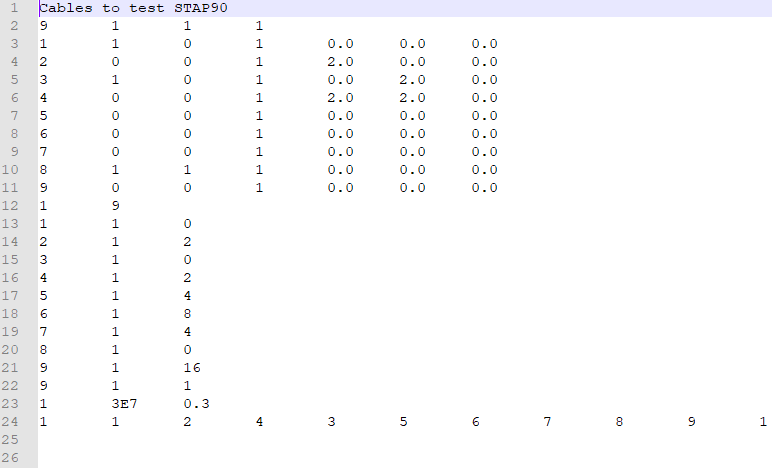
\includegraphics[width = .8\textwidth]{8.png} 
\caption{1个9节点亚参元的输入文件格式} 
\label{f8} 
\end{figure}

\subsection{分片测试}

先考虑考虑一个平板的一端(沿着xy平面),长宽:$W=L=2$,其材料参数:$E=3\times10^{7},\nu=0.3$,其受到$x$方向的一个均匀拉力$\sigma=9$的情况,如图\ref{f9}所示:

\begin{figure}[H]
\centering  
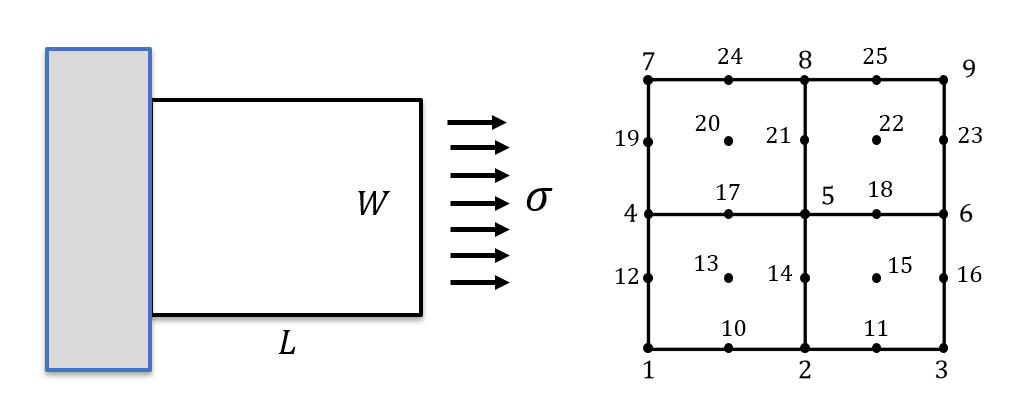
\includegraphics[width = .5\textwidth]{9.png} 
\caption{9节点平面亚参元的分片测试1示意图} 
\label{f9} 
\end{figure}并且我们划分4个等大的单元,节点划分如图\ref{f9}所示,其中平板的一段被约束住(即节点1,7,12,19被约束住$x$方向自由度,而4号节点约束住$x,y$方向自由度);利用节点力等效公式(\ref{eq26})我们可以得到在该情况下(对于矩形单元)的节点等效力为:$f_{ix}|_{\Gamma}=\frac{\sigma h}{2}\int_{-1}^{1}N_{i}(\xi=1){\rm d\eta}$(其中$h$为单元的长度)

\begin{equation}
\begin{array}{c}
f_{2x}=f_{4x}=\frac{1}{6}\sigma h\\
f_{6x}=\frac{2}{3}\sigma h
\end{array}\label{eq27}
\end{equation}
注意这里的1-9对应的是母单元的编号,具体的编号要根据Location matrix对应的世纪编号来;相应的具体输入文件利用matlab程序Subpara\_force.m生成,具体输入文件请见Subparapatchtest.dat,程序计算的求解结果如图\ref{f10}所示:

\begin{figure}[H]
\centering  
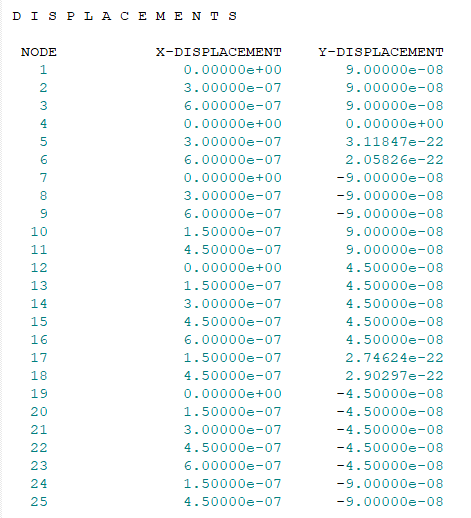
\includegraphics[width = .5\textwidth]{10.png} 
\caption{9节点平面亚参元的分片测试1结果} 
\label{f10} 
\end{figure}其与理论的结果(单轴拉伸):

\begin{equation}
\begin{array}{c}
u=\frac{\sigma}{E}x\\
v=-\frac{\nu\sigma}{E}(y-1)
\end{array}\label{eq28}
\end{equation}
相比较,从5号节点的$y$方向位移,可以看出其误差基本在计算机浮点数范围$(10^{-22})$内,因此通过分片测试1;

进一步的提高分片测试的阶次,给平板一个沿着$x$方向均匀拉伸的体积力$b_{x}=a=9$,其余参数不变,如图\ref{f11}所示:

\begin{figure}[H]
\centering  
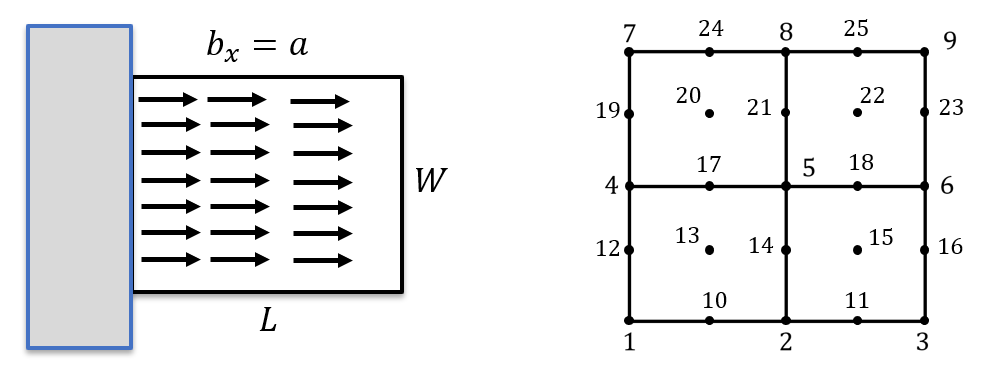
\includegraphics[width = .5\textwidth]{11.png} 
\caption{9节点平面亚参元的分片测试1示意图} 
\label{f11} 
\end{figure}

同样利用节点力等效公式(\ref{eq26}),我们可以得到(对于矩形单元)每个单元等效的节点力为:$f_{ix}=\frac{ah^{2}}{4}\int_{-1}^{1}\int_{-1}^{1}N_{i}{\rm d}\xi{\rm d\eta}$(其中$h$为单元的长度)

\begin{equation}
\begin{array}{c}
f_{1x}=f_{2x}=f_{3x}=f_{4x}=\frac{ah^{2}}{36}\\
f_{5x}=f_{6x}=f_{7x}=f_{8x}=\frac{ah^{2}}{9}\\
f_{9x}=\frac{4ah^{2}}{9}
\end{array}\label{eq29}
\end{equation}
其余的输入文件文件部分和Subparapatchtest.dat相同,见Subparapatchtest2.dat文件;程序的计算求解结果如图\ref{12}所示:

\begin{figure}[H]
\centering  
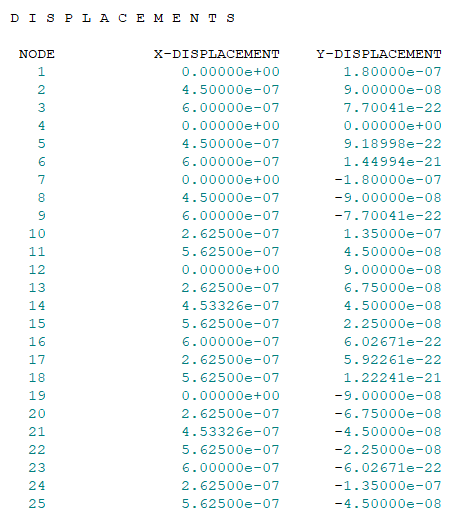
\includegraphics[width = .5\textwidth]{12.png} 
\caption{9节点平面亚参元的分片测试2结果} 
\label{f12} 
\end{figure}其与理论结果:

\begin{equation}
\begin{array}{c}
u=\frac{a}{E}(2x-\frac{x^{2}}{2})\\
v=-\frac{a\nu}{E}(2-x)(y-1)
\end{array}\label{eq30}
\end{equation}
比较的误差在计算浮点数范围$(10^{-22})$,因此其能通过分片测试2,所以其收敛率至少为3。

\subsection{收敛率计算}

将分片测试2中的均匀体积力改为一个沿 $x$方向线性分布体力的情况:$b_{x}=ax(a=9)$,其余几何参数,材料参数以及单元划分不变,如图\ref{f13}所示:

\begin{figure}[H]
\centering  
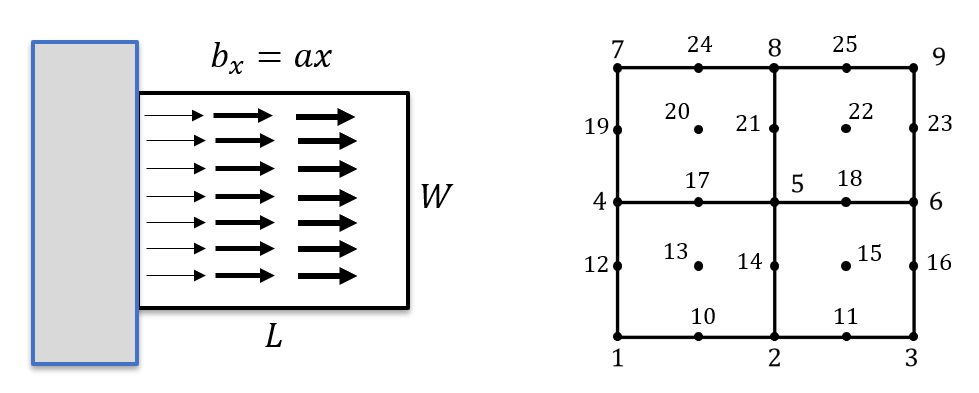
\includegraphics[width = .5\textwidth]{13.png} 
\caption{9节点平面亚参元收敛率计算示意图} 
\label{f13} 
\end{figure}

同样利用节点力等效公式(\ref{eq26}),我们可以得到(对于矩形单元)每个单元等效的节点力为:$f_{ix}=\frac{ah^{2}}{4}\int_{-1}^{1}\int_{-1}^{1}N_{i}{\rm (\frac{x_{1}+x_{2}}{2}+\frac{h}{2}\xi)d}\xi{\rm d\eta}$(其中$x_{1}$和$x_{2}$为母单元中1,2号节点对应物理空间的坐标,$h$为单元长度)

\begin{equation}
\begin{array}{c}
f_{1x}=f_{4x}=\frac{ah^{2}}{36}(\frac{x_{1}+x_{2}}{2}-\frac{h}{2})\\
f_{2x}=f_{3x}=\frac{ah^{2}}{36}(\frac{x_{1}+x_{2}}{2}+\frac{h}{2})\\
f_{5x}=f_{7x}=\frac{ah^{2}}{9}\frac{x_{1}+x_{2}}{2}\\
f_{6x}=\frac{ah^{2}}{9}(\frac{x_{1}+x_{2}}{2}+\frac{h}{2})\\
f_{8x}=\frac{ah^{2}}{9}(\frac{x_{1}+x_{2}}{2}-\frac{h}{2})\\
f_{9x}=\frac{4ah^{2}}{9}\frac{x_{1}+x_{2}}{2}
\end{array}\label{eq31}
\end{equation}
注意这里的1-9对应的是母单元的编号,具体的编号要根据Location matrix对应的世纪编号来;相应的具体输入文件利用matlab程序Subpara\_force.m生成;我们分别计算划分1,4,16和64个单元时的结果(对应单元尺寸$h=2,1,0,5,0.25$),具体输入文件请见Subpara1ele.dat,Subpara4ele.dat,Subpara16ele.dat和Subpara64ele.dat;计算相应的节点位移$w^{e}$与理论结果进行比较:

\begin{equation}
\begin{array}{c}
u=\frac{3}{2E}(12x-x^{3})\\
v=\frac{9\nu}{2E}(x^{2}-4)(y-1)
\end{array}\label{eq32}
\end{equation}
我们这里计算$x$方向位移的误差范数:

\begin{equation}
error=(\int_{0}^{L}\int_{0}^{W}(u^{e}-u)^{2}dxdy)^{\frac{1}{2}}\label{eq33}
\end{equation}
由于$u$是三次场,所以至少要用9{*}9节点Gauss积分,得到的计算结果如图\ref{f14}所示:

\begin{figure}[H]
\centering  
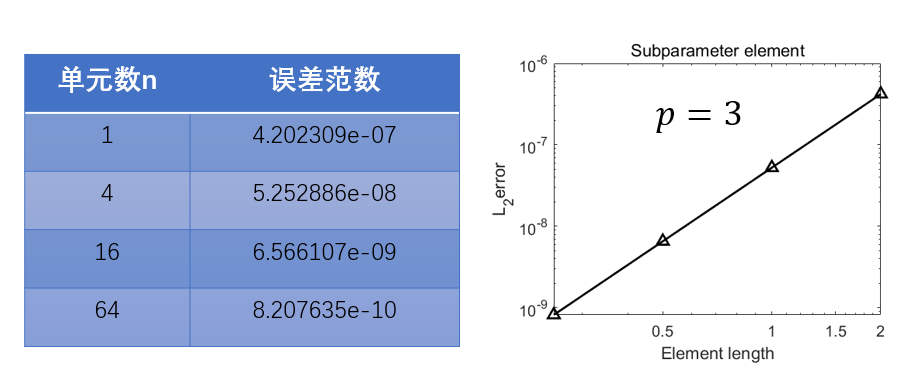
\includegraphics[width = .5\textwidth]{14.png} 
\caption{9节点平面亚参元收敛率计算结果} 
\label{f14} 
\end{figure}可见其位移的收敛率为3,和分片实验的结果一致,因为其位移差值能够精确重构2次多项式。

\section{无限单元(Infinite element)}

\subsection{无限单元的基本公式}

我们这里采用的是4节点平面等参无限单元(之后简称为无限单元);其主要适用于无限大问题的求解,其核心的思想是利用两个参考点$\text{{\rm C}}$和${\rm C_{1}}$把边界点${\rm P}$和${\rm P_{1}}$还有对称的参考点$\text{{\rm Q}和\ensuremath{{\rm Q_{1}}\text{把无穷原点映射到母单元中\ensuremath{\xi=1}}}}$的两个点;最终在母单元中${\rm P},{\rm Q},{\rm R}$和${\rm P}_{1},{\rm Q_{1}},{\rm R_{1}}$对应平行与$\xi$轴的两条边,因此我们只需要构造一种一维差值$(\xi\text{方\text{向}})$能够满足把无穷远R点$(x\to\infty)$映射到$\xi=1$即可,如图\ref{f15}所示:

\begin{figure}[H]
\centering  
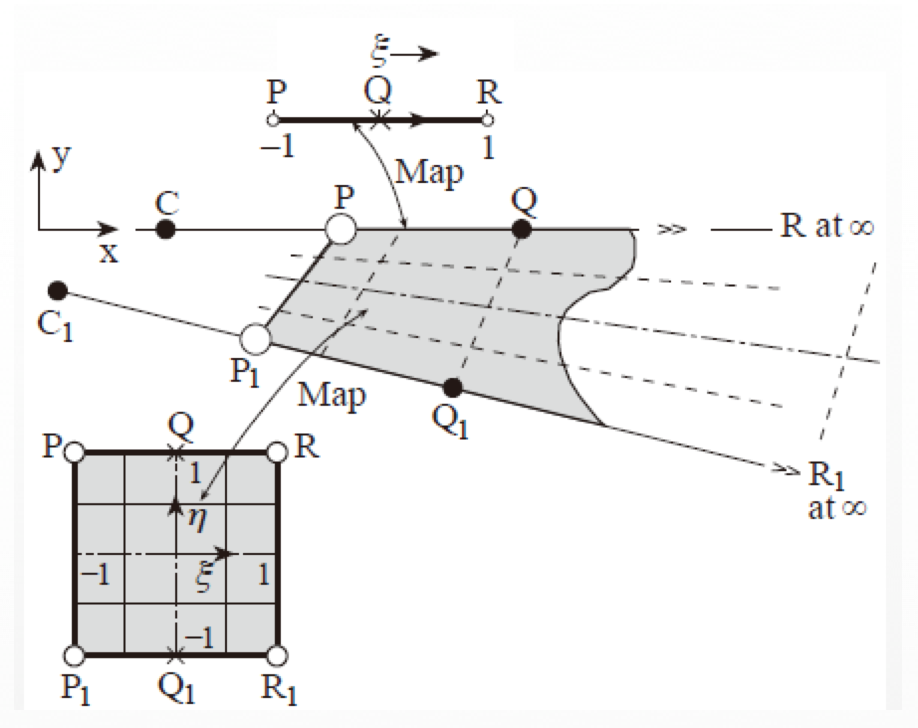
\includegraphics[width = .6\textwidth]{15.png} 
\caption{无限单元映射关系示意图} 
\label{f15} 
\end{figure}首先对于$\xi$方向的差值:

\begin{equation}
\begin{array}{c}
x=\text{\ensuremath{\overline{N}_{C}x_{C}+\overline{N}_{Q}x_{Q}}}\\
\overline{N}_{C}=-\frac{\xi}{1-\xi}\\
\overline{N}_{Q}=1+\frac{\xi}{1-\xi}
\end{array}\label{eq34}
\end{equation}
其可以使得P点从物理空间中的$x=\frac{x_{C}+x_{Q}}{2}$映射到$\xi=-1$,使得Q点从物理空间中的$x=x_{Q}$映射到$\xi=0$,使得R点从物理空间中的$x\to\infty$映射到$\xi=1$,而$\eta$方向的差值可直接采用一般的两节点线性差值:$N_{1}=\frac{1}{2}\eta(1+\eta),N_{0}=\frac{1}{2}\eta(1-\eta)$,于是整个4节点无限单元的形函数和差值关系为:

\begin{equation}
\begin{array}{c}
x=\sum_{i=1}^{4}N_{i}^{*}x_{i}\\
N_{1}^{*}=N_{1}(\eta)\overline{N}_{C}\\
N_{2}^{*}=N_{1}(\eta)\overline{N}_{Q}\\
N_{3}^{*}=N_{0}(\eta)\overline{N}_{C}\\
N_{4}^{*}=N_{0}(\eta)\overline{N}_{Q}
\end{array}\label{eq35}
\end{equation}
其中$i=1$对应C,$i=2$对应Q,$i=3$对应${\rm C_{1}}$,$i=4$对应$Q_{1}$。

\subsection{无限单元的应力应变以及刚度阵构造}

其余有关应力和刚度阵的后续推导和平面4节点等参元一致,但是由于形函数不同(分式多项式),会导致形函数的导数会有变化:

\begin{equation}
\begin{array}{ll}
{\frac{\partial N_{1}^{*}}{\partial\xi}=-\frac{1}{2}\frac{(1+\eta)}{(1-\xi)^{2}}} & {\frac{\partial N_{1}^{*}}{\partial\eta}=-\frac{1}{2}\frac{\xi}{1-\xi}}\\
{\frac{\partial N_{2}^{*}}{\partial\xi}=\frac{1}{2}\frac{(1+\eta)}{(1-\xi)^{2}}} & {\frac{\partial N_{2}^{*}}{\partial\eta}=\frac{1}{2}\left(1+\frac{\xi}{1-\xi}\right)}\\
{\frac{\partial N_{3}^{*}}{\partial\xi}=-\frac{1}{2}\frac{(1-\eta)}{(1-\xi)^{2}}} & {\frac{\partial N_{3}^{*}}{\partial\eta}=\frac{1}{2}\frac{\xi}{1-\xi}}\\
{\frac{\partial N_{4}^{*}}{\partial\xi}=\frac{1}{2}\frac{(1-\eta)}{(1-\xi)^{2}}} & {\frac{\partial N_{4}^{*}}{\partial\eta}=-\frac{1}{2}\left(1+\frac{\xi}{1-\xi}\right)}
\end{array}\label{eq36}
\end{equation}
从而代入到$\bm{B}$矩阵的计算中:

\begin{equation}
\begin{array}{cc}
[\boldsymbol{B}]=\left[\begin{array}{cc}
{\frac{\partial N_{i}^{*}}{\partial x}} & {0}\\
{0} & {\frac{\partial N_{i}^{*}}{\partial y}}\\
{\frac{\partial N_{i}^{*}}{\partial y}} & {\frac{\partial N_{i}^{*}}{\partial x}}
\end{array}\right]=[J]^{-1}\left[GN^{*}\right] & [\mathbf{J}]=\left[\begin{array}{cc}
{\frac{\partial x}{\partial\xi}} & {\frac{\partial y}{\partial\xi}}\\
{\frac{\partial x}{\partial\eta}} & {\frac{\partial y}{\partial\eta}}
\end{array}\right]\end{array}\label{eq37}
\end{equation}
进一步由公式(\ref{eq25})计算刚度阵列,程序中采用$2\times2$的Gauss积分(但是由于这里雅可比矩阵中存在分式多项式,因此Gauss积分不一定能够做到准确积分)计算并且用Skyline的方式存储。

而其余的节点力等效和Gauss点应力计算和4Q单元一致,程序实现上的思路也一致,只是需要把形函数改为(\ref{eq35})

\subsection{无限单元的收敛性分析}

首先无限单元作为物理尺寸无限大的单元无法像常规的单元一样用单元的尺寸来考虑收敛率,但是从等参元的基本性质出发,无限单元是满足等参元的相容性和连续性:(因为其对应的节点C,Q不是有限单元边界上的点P),于此同时其同样满足刚体位移条件:

\begin{equation}
\sum_{i=1}^{4}N_{i}^{*}=1\label{eq38}
\end{equation}
因此该单元是收敛的。但是需要注意,由于无限单元节点的特殊性,这使得输入文件的构造变得很困难,首先需要给定有限单元的边界,然后去寻找关于边界的对称点,这对于程序上实现会有一些难度。
\end{document}
